% Automatically generated figure environments; include graphics relative to paper.tex.
\begin{figure}[t]
\centering
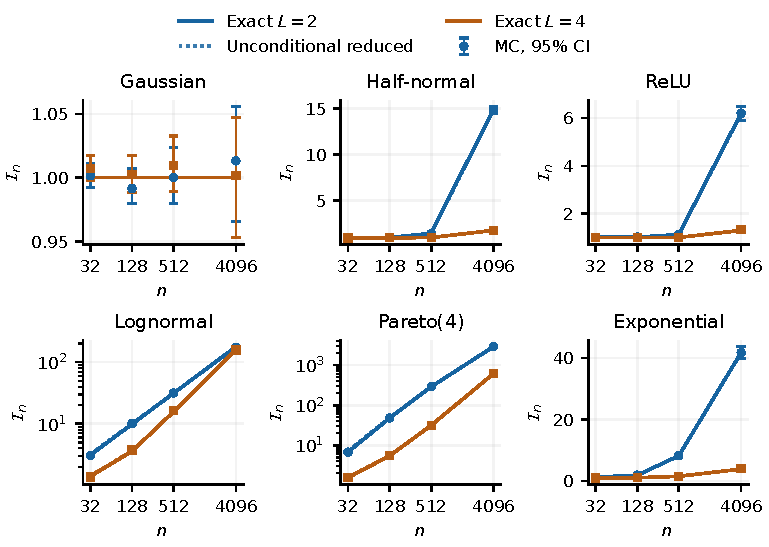
\includegraphics[width=\linewidth]{revision/experiments/figure_benchmark.pdf}
\caption{Finite-block validation on six input laws. Solid curves are exact moment predictions; dotted curves use unconditional responses and drop conditional covariance. Markers show Monte Carlo estimates with 95\% intervals, using conditional stratification for Pareto.}\label{fig:revision-benchmark}
\end{figure}
\begin{figure}[t]
\centering
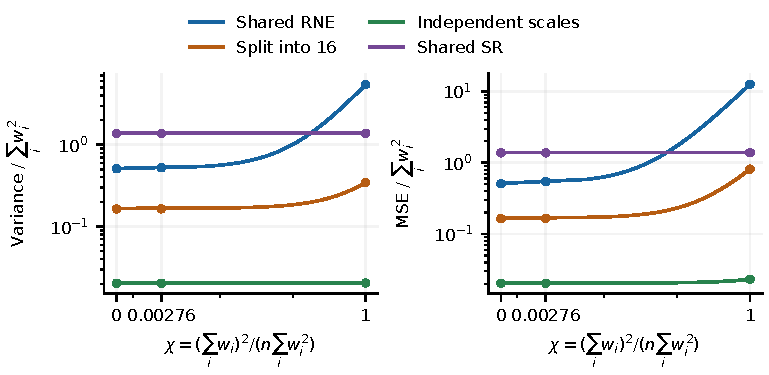
\includegraphics[width=\linewidth]{revision/experiments/figure_weighted.pdf}
\caption{Weighted dot products for lognormal inputs ($n=128$, $L=2$). Fixed weights vary the normalized imbalance $\chi=(\sum_iw_i)^2/(n\sum_iw_i^2)\in[0,1]$. Curves evaluate the affine laws from exact moments on a dense grid; markers show Monte Carlo with 95\% intervals.}\label{fig:revision-weighted}
\end{figure}
\begin{figure}[t]
\centering
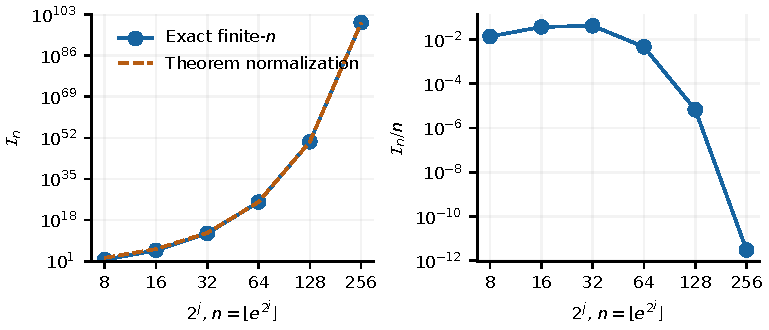
\includegraphics[width=\linewidth]{revision/experiments/figure_exponential.pdf}
\caption{Exponential inputs provide unbounded variance inflation on a dyadic subsequence despite $\mathcal I_n/n\to0$. Values use exact exponent probabilities and 160-digit cell integration, independently checked at 100 digits.}\label{fig:revision-exponential}
\end{figure}
